\section{Introdução}\label{sec:introducao}

% - Qual é a da coisa? (sintese c webaudio)
% - como a coisa funciona? 
%   - como um ou outro fez funcionar
%   - nosso jeito de funcionar

% -----------------------------------------------
 % http://www.charlie-roberts.com/pubs/Gibber_charles_roberts_icmc_2012.pdf


O processamento de sinais digitais de áudio em navegadores de rede, é sumarizado por \cite{w3c_web_2012,roberts_web_2013-,wyse_viability_2014}. \cite{srikumar_tamming_2013} exemplifica a utilização de \emph{nós de áudio}, que podem ser concatenados em um grafo de DSP, como três instâncias de nós diferentes -- \emph{OscilatorNode}, \emph{GainNode}, \emph{DestinationNode} --, na Figura \ref{fig:shime}. Existe um outro nó, \emph{ScriptProcessorNode} que possibilita a customização de funções sonoras. Este último foi utilizado no desenvolvimento do \emph{Termpot}.

\begin{figure}[h]
\centering
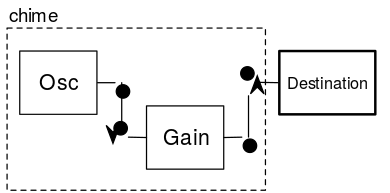
\includegraphics[scale=0.35]{chime.png}
\caption{Estrutura básica de síntese da API webaudio, utilizando instâncias das classes \emph{OscilatorNode}, \emph{GainNode}, \emph{DestinationNode}. \textbf{Fonte}: \cite{srikumar_tamming_2013}.}
\label{fig:shime}
\end{figure}

\section{Trabalho relacionado: GROOVE}

Este artigo envolve a utilização  tecnologia \emph{Web Audio}, e de seu nó \emph{ScriptProcessorNode}, sob uma perspectiva histórica. Neste sentido, o trabalho de \cite{mathews_groove_1970}, GROOVE \emph{Generated Real-time Operations On Voltage-controlled Equipment},foi fundamental para a estruturação do \emph{Termpot}. Um humano digita comandos em um computador, que são renderizados em som. O som, por sua vez, será percebido pela pessoa, que fornecerá uma nova entrada de dados (através de novos comandos, ou dispositivos, como controles manuais). O processo de síntese sonora considera, portanto, questões performáticas, como a imediaticidade. Um exemplo de música feita com o GROOVE, como apresentado na figura \ref{fig:groove}, é a obra \emph{The Expanding Universe} de \cite{spiegel_expanding_1975} \footnote{Disponível em \url{https://www.youtube.com/watch?v=dYUZmsfm4Ww}.}.

\begin{figure}[!h]
  \begin{center}
  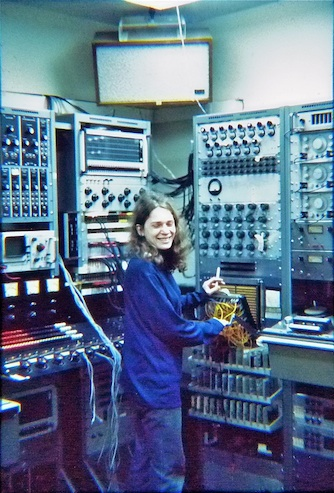
\includegraphics[scale=0.5]{./spiegel.jpg}
  \caption{Laurie Spiegel configurando a saída analógica do GROOVE, durante a produção de \emph{The Expanding Universe}. \textbf{Fonte}: \cite{spiegel_expanding_1975}.}
  \label{fig:groove}
  \end{center}
\end{figure}

\section{Objetivo}

Descrever um programa \emph{web} desenvolvido com base no \emph{ScriptProcessorNode}, e estruturado segundo uma interpretação GROOVE.

%A Seção \ref{sec:trabalhos} deste artigo apresenta os frameworks supracitados e uma breve comparação entre eles.
%A Seção \ref{sec:termpot} apresenta a ferramenta proposta.
%A Seção \ref{sec:resultados} traz os resultados desta pesquisa e a Seção \ref{sec:conclusao} apresenta as conclusões do trabalho até o presente momento.

\section{Metodologia de desenvolvimento}

Para a implementação, três tarefas foram necessárias: \begin{inparaenum}[\itshape 1)\upshape]
\item Customização um emulador terminal: foi utilizada a biblioteca \emph{Ptty.js}\footnote{Disponível em \url{http://code.patxipierce.com/jquery-plugin/ptty/}.}
\item Definição de um ambiente interno customizado, no \emph{ScriptProcessorNode}, como utilizado pelo ambiente \emph{Wavepot}\footnote{Disponível em \url{http://www.wavepot.com}.}.
\item Definição de comandos deste ambiente interno: inspeção de funções, definição de novas funções, tocar, parar, pausar, gravar e download, criação de controles gráficos (\emph{jQueryUI}) e gravação\footnote{Disponível em \url{https://github.com/mattdiamond/Recorderjs/blob/master/recorderWorker.js}.}.
\end{inparaenum}

